
\section{The Age-\oh~Relation} 
\label{migration:sec:age_oh_relation}

% fig 18 
\begin{figure*} 
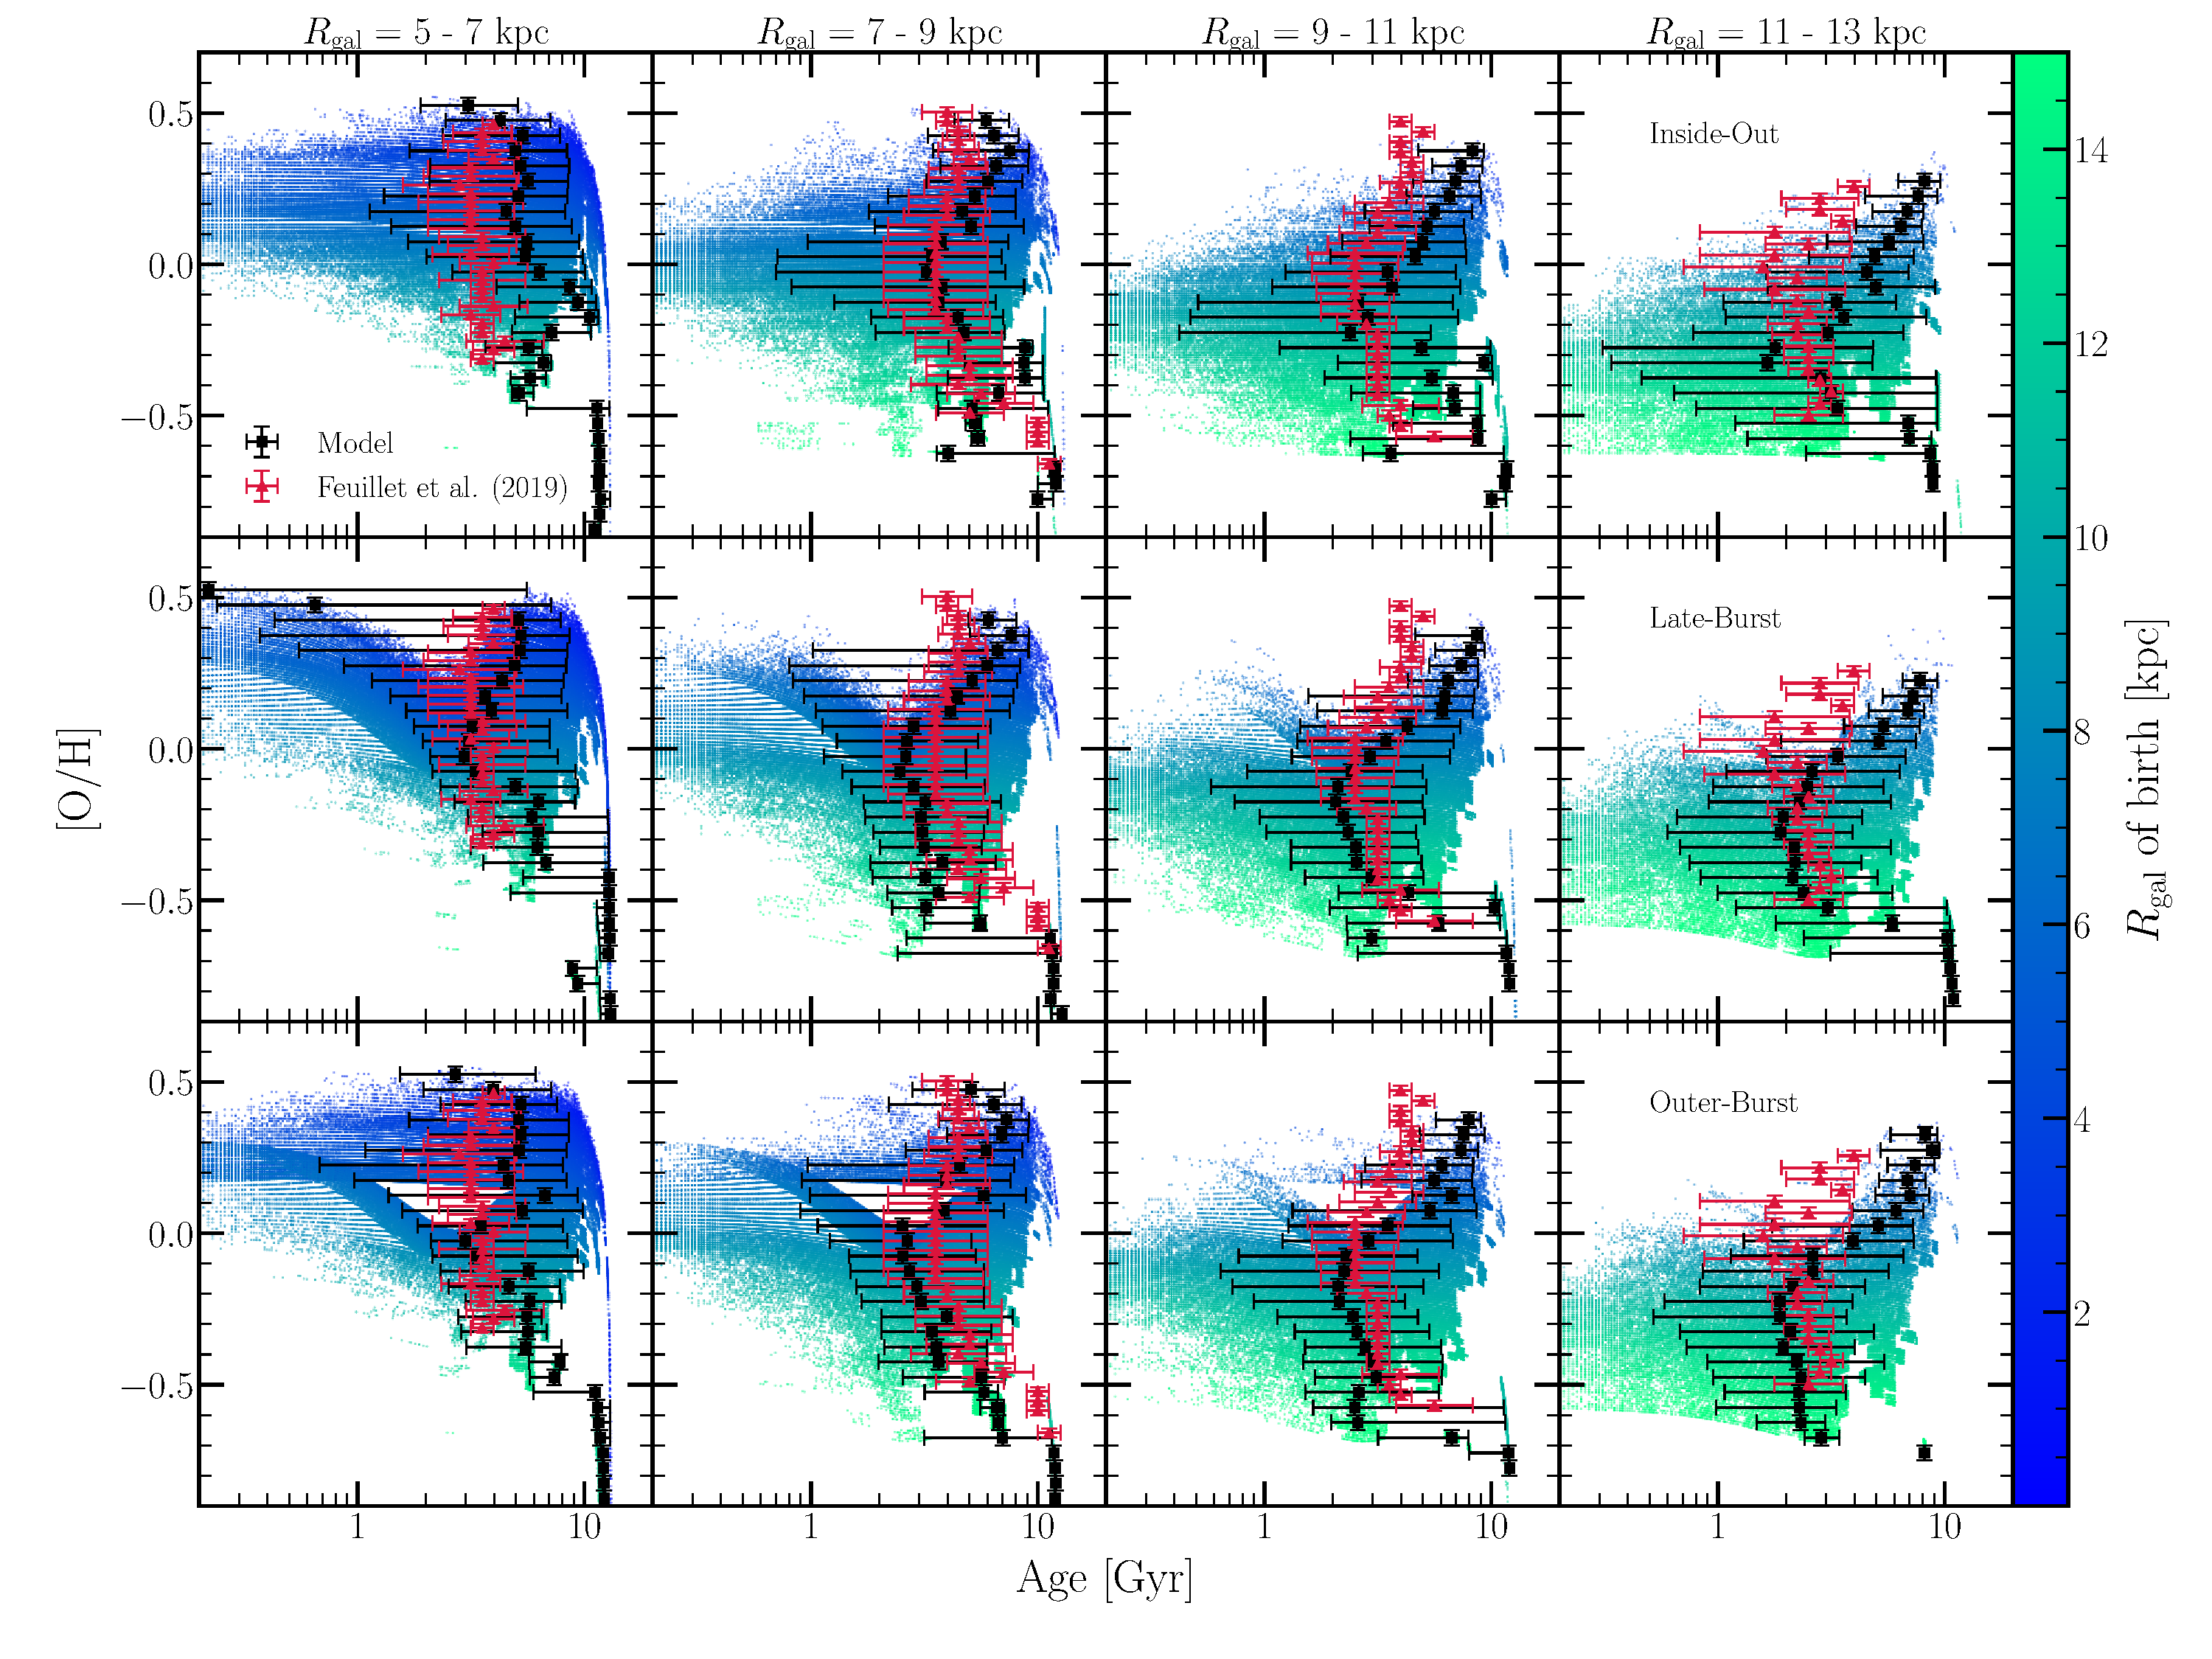
\includegraphics[scale = 0.32]{chapter5/age_oh_comparison.pdf} 
\caption{The same as Fig.~\ref{migration:fig:amr_insideout_vs_lateburst_fe}, but for 
\oh, and with an additional comparison to the outer-burst model in the 
bottom row.} 
\label{migration:fig:age_oh_comparison} 
\end{figure*} 

Fig.~\ref{migration:fig:age_oh_comparison} presents a comparison of the age-\oh~ 
relation predicted by our inside-out, late-burst, and outer-burst SFHs to 
the~\citet{Feuillet2019} measurements in the same Galactic regions as in 
Fig.~\ref{migration:fig:amr_insideout_vs_lateburst_fe}. 
The age-\oh~relation shows a smoother population-averaged trend than the 
age-\feh~relation (see Fig.~\ref{migration:fig:amr_insideout_vs_lateburst_fe}). 
Affected by the variability in Type Ia supernova rates discussed in 
\S~\ref{migration:sec:obs_comp:gradient}, the gas-phase Fe abundance at fixed radius 
fluctuates as a function of simulation time, resulting in higher intrinsic 
scatter in the age-\feh~relation than in age-\oh. 
We can make similar arguments about the age-\oh~relation as we do for 
age-\feh~in~\S~\ref{migration:sec:obs_comp:amr}: the late-burst model better reproduces 
the C-shaped nature of the AMR throughout the disc, particularly beyond the 
solar neighbourhood. 
The bin-by-bin comparison is also somewhat more convincing in age-\oh~than in 
age-\feh. 
The late-burst model improves the agreement in all annuli with the exception of 
the solar annulus, where it potentially worsens the agreement slightly, but 
both models adequately reproduce the data there anyway. 
% \par 
In comparing the late-burst model to the outer-burst model, it is clear the 
outer-burst model mitigates the very young ages of the most metal-rich stars 
at~\rgal~= 5 - 7 kpc seen in the late-burst model; this is a consequence of 
the starburst producing a bimodal age distribution at these abundances (see 
discussion in~\S~\ref{migration:sec:obs_comp:amr}). 

